\documentclass[a4paper]{article}
\usepackage{exercise}
%um nur aufgaben zu zeigen
%\usepackage[noanswer]{exercise} 
\usepackage{../images/preamble}
\usepackage{rotating}
\usetikzlibrary{decorations.pathmorphing}
\pagestyle{fancy}
\fancyhead[L]{\includegraphics[width=2cm]{../images/logo_scaled.pdf}}
\fancyhead[R]{\textsc{Lösung Aufgabenserie 2}}
\begin{document}
%	\vspace*{-2cm}
%	\parbox{4cm}{\includegraphics[width=2.5cm]{../images/ROLF4.png}}
%	\parbox{10.6cm}{\setstretch{2.0} \centering{ \huge \textsf{Aufgabenserie 2}}\\ Abgabe: 19. Juni \\ \vspace*{-.5cm} }
\vspace*{-1cm}
\parbox{4cm}{\vspace{-0.2cm}\includegraphics[width=5cm]{../images/logo_scaled.pdf}}
\parbox{10.6cm}{\setstretch{2.0} \centering{ \huge \textsf{Aufgabenserie 2 
		}}\\
		Abgabe: 19. Juni 2017 \\ \vspace*{-.5cm} }
	\vspace{0.5cm}	
	

\thispagestyle{empty}
\begin{framed}
	\noindent
	\scriptsize
	Die Aufgaben sollten bis zum \textbf{19. Juni} bearbeitet werden. Die Lösungen schickt ihr an \href{mailto:physikrolf@gmail.com}{physikrolf@gmail.com}.
	Jede Aufgabe hat eine bestimmte Anzahl an erreichbaren Punkten. Wie viele das sind, müsst ihr raten. Versucht, die Lösungen so genau wie möglich aufzuschreiben. Für besonders schnelle/gute/witzige Lösungen kann es Bonuspunkte geben.\\ Die aktuellen Aufgaben sowie alle alten Aufgabenserien mit Lösungen findet ihr auch auf \url{pankratius.github.io/rolf}
\end{framed}

\noindent
\begin{Exercise}[label = hypercube, origin = Aaron Wild, difficulty = 5, title =  Widerstandswürfel]
Ein $n$-dimensionaler Hyperwürfel ist die Verallgemeinerung eines Würfels auf $n$ Dimensionen. Seine Konstruktion kann man sich so vorstellen, das ein $n-1$-dimensionaler Hyperwürfel im $n$-dimensionalen Raum parallelverschoben wird, und man das daraus entstandene Volumen betrachtet.\\
Ein solcher $n$-dimensionaler Hyperwürfel hat $2^n$ Eckpunkte und $n2^{n-1}$ Seitenkanten.\\
Wir betrachten nun einen $n$-dimensionalen Hyperwürfel ($n\geq 1$), bei dem alle Seitenkanten einen Widerstand von $r$ haben. Zeige, dass der Widerstand zwischen zwei benachbarten Eckpunkten 
\begin{equation}
	R = \frac{2-2^{1-n}}{n}r = \frac{2^n-1}{n2^{n-1}}r
\end{equation}
beträgt. Überlege dir an einem $n$ deiner Wahl, dass das Ergebnis dort sinnvoll ist.
\end{Exercise}
\begin{Exercise}[label=heate, origin = {US IPhO Auswahlwettbewerb, Halbfinale 2013}, title = Wärmetauscher]
Die durch Wärmeleitung übertragene Wärmeleistung zwischen zwei parallelen Wänden kann näherungsweise durch die Gleichung 
\begin{equation}\label{he:fg}
	P = \lambda A \frac{T_a-T_b}{d}
\end{equation}
beschrieben werden. Dabei ist $A$ die Fläche, durch die Wärme strömt, $d$ der Abstand zwischen den beiden Wänden und $\lambda$ eine Konstante, die vom Material zwischen den beiden Wänden abhängt (die sog. Wärmeleitfähigkeit). $T_a$ ist die Temperatur der wärmeren Wandoberfläche und $T_b$ die der kälteren Wandoberfläche.\\
Ein Wärmetauscher ist ein Gerät, dass Wärme von einer warmen Flüssigkeit zu einer kälteren Flüssigkeit überträgt (Abb. \ref{fig:heate}).
Dabei fließt warme Flüssigkeit (rot) mit einer Geschwindigkeit $v$ von rechts nach links, und kalte Flüssigkeit (blau) mit einer Geschwindigkeit von $v$ von links nach rechts. Die Dichte der Flüssigkeiten ist $\rho$ und die Wärmekapazität $c$. Beide befinden sich in Röhren der Höhe $h$ ($h$ ist sehr klein).  Die beiden Flüßigkeiten sind durch eine Metallwand (grau) der Dicke $d$ mit der Wärmeleitfähigkeit $\lambda$ getrennt. \\
Die Temperaturdifferenz zwischen der einfließenden warmen Flüssigkeit und der einfließenden kalten Flüssigkeit beträgt $\Delta T_e$. \\
Bestimme die Temperaturdifferenz zwischen der abgekühlten, ausfließenden warmen Flüssigkeit und der aufgewärmten, ausfließenden kalten Flüßigkeit, $\Delta T_a$. Nimm dafür an, dass die Temperaturdifferenz $\Delta T$ zwischen warmer und kalter Flüssigkeit entlang der Wand konstant bleibt.

\end{Exercise}
\begin{figure}[h]
	\centering
	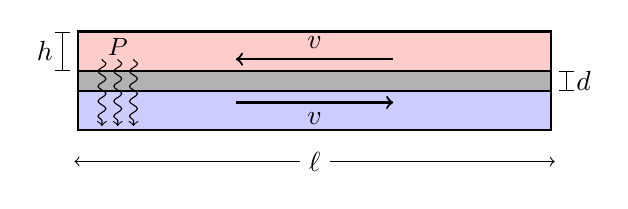
\begin{tikzpicture}

\filldraw[thick, draw = black, fill = red!20!white] (-3,-0.25)rectangle (3,.25);
\filldraw[thick, draw = black, fill= black!30!white] (-3,-0.5)rectangle (3,-.25);
\filldraw[thick,draw= black, fill=blue!20!white] (-3,-1)rectangle(3,-.5);

\draw[|-|] (3.2,-.25)--(3.2,-.5) node [midway, right] {$d$};

\draw[->,thick] (-1,-.65) -- (1,-.65) node[midway, below] {$v$};
\draw[<-,thick] (-1,-.1)--(1,-.1) node[midway, above]{$v$};
\draw[->,decorate,decoration={snake, amplitude = 0.5mm, segment length = 1.9mm}] (-2.5,-0.1) -- (-2.5,-.95);
\draw[->,decorate,decoration={snake, amplitude = 0.5mm, segment length = 1.9mm}] (-2.7,-0.1) -- (-2.7,-.95);
\draw[->,decorate,decoration={snake, amplitude = 0.5mm, segment length = 1.9mm}] (-2.3,-0.1) -- (-2.3,-.95);
\node at (-2.5,0.05) {\small $P$};
\draw[|-|] (-3.2,.25)--(-3.2,-.25) node[midway, left]{$h$};
\draw[<->] (-3.05,-1.4) -- (3.05,-1.4) node[midway, fill = white] {$\ell$};
\end{tikzpicture}
	\caption{Ein Wärmetauscher}
	\label{fig:heate}
\end{figure}
\begin{minipage}[b]{0.8\textwidth}
\noindent
\begin{Exercise}[label = can, title = {Büchse}, origin = {nach 3. Runde IPhO, 2011},difficulty = 1]
	Bestimme die Position des Schwerpunkts $h_s$ einer gefüllten zylinderförmigen Büchse in Abhängigkeit der Füllhöhe $h_f$ und der relevanten Parameter. Nimm dafür an, dass die Büchse eine gleichmäßige Massenverteilung hat. 
\end{Exercise}
\end{minipage}
\begin{minipage}[b]{0.2\textwidth}
\centering
\begin{tikzpicture}
\draw (-0.5,1)--(-0.5,0)--(0.5,0)--(0.5,1);
\fill[pattern = north east lines] (-0.5,0.6)--(-0.5,0)--(0.5,0)--(0.5,0.6);
\filldraw[black] (0,0.3) circle (2pt);
\draw[<->] (0.7,0) -- (0.7,0.3) node[midway, right]{$h_s$} ;
\draw[<->] (-0.7,0) -- (-0.7,0.6) node[midway, left]{$h_f$};

\end{tikzpicture}
\end{minipage}
\begin{Answer}[ref = can]
	Weil die Büchse eine gleichmäßige Massenverteilung hat, und wir auch annehmen können, dass die Flüssigkeit eine gleichmäßige Dichte hat, muss das System rotationssymetrisch um die senkrechte Achse durch den Deckel und den Boden sein. Das heißt aber nichts anderes, als das eine Drehung der Büchse um diese Achse keine messbaren Unterschiede hervorbringen kann, weshalb der Schwerpunkt in auf dieser Achse liegen muss. Wäre das nämlich nicht so, gäbe es eine Möglichkeit, festzustellen, wie die Büchse um diese Achse gedreht wurden ist, welche es aber wegen der Rotationssymetrie nicht geben darf.\\
	Die Höhe des Schwerpunkts kann man nun am Einfachsten über die Definitionsgleichung bestimmen. Dafür stellen wir uns das System zusammengesetzt aus der Flüssigkeit und der Büchse vor. Der Schwerpunkt der Büchse liegt bei $h_{Sp,b} = \frac{h_b}{2}$, wobei $h_b$ die Höhe der Büchse ist, und der der Flüssigkeit liegt bei $h_{Sp,f}=\frac{h_f}{2}$. Die Höhe $h$ des Gesamtschwerpunkts (relativ zum Boden der Büchse) ist gegeben durch
	\begin{equation}\label{can:spdef}
		h = \frac{m_{b}h_{Sp,b}+m_{f}h_{Sp,f}}{m_{b}+m_{f}},
	\end{equation}
	wobei $m_b = \rho_b h_b$ die Masse der Büchse ist, und $m_f = \rho_f h_f$ die Masse der Flüßigkeit. Setzt man diese beiden Ausdrücke in \eqref{can:spdef} ein, so erhält man
\end{Answer}





%
%\newpage
%\begin{turn}{270}
%\definecolor{qqttcc}{rgb}{0.,0.2,0.8}
\definecolor{ffqqqq}{rgb}{1.,0.,0.}
\definecolor{ffqqtt}{rgb}{1.,0.,0.2}
\definecolor{cqcqcq}{rgb}{0.7529411764705882,0.7529411764705882,0.7529411764705882}
\begin{tikzpicture}[line cap=round,line join=round,>=triangle 45,x=0.75cm,y=0.75cm]
\draw [color=cqcqcq,, xstep=1.5cm,ystep=1.5cm] (-8.5,0.6) grid (23.,20.);
\clip(-8.5,0.6) rectangle (23.,20.);
\draw (-5.588239388018447,9.518801182219294) node[anchor=north west] {$S$};
\begin{scriptsize}
\draw [fill=black] (-5.65741495087795,9.439855831290508) circle (2.5pt);
\draw [fill=ffqqtt] (1.9550099267845686,14.114279339778834) circle (2.0pt);
\draw [fill=ffqqqq] (17.86598524604952,10.425615052655644) circle (2.0pt);
\draw [fill=qqttcc] (2.6268608640983873,14.364446314147006) circle (2.0pt);
\draw [fill=qqttcc] (18.279983363360785,9.990865906507295) circle (2.0pt);
\end{scriptsize}
\end{tikzpicture}
%\end{turn}



\end{document}
